\chapter{Background}
\label{chp:background} 

\noindent This thesis describes the setup and usage of an end-to-end \gls{iot} system. In order for the testbed to be set up and reproduced by others, a detailed description of components, sensors and protocols used, is provided. This chapter will undergo the background information of the devices, technologies and protocols used, and why these were chosen over other alternatives.  
%\todo{Add example? }
%\section{Internet of Things} % Tjae

%Comment: Read Future Internet: The Internet of Things from 2010.  \cite{gubbi2013internet}

%Comment: Read http://ac.els-cdn.com/S1570870512000674/1-s2.0-S1570870512000674-main.pdf?_tid=6f15526e-eae8-11e5-addc-00000aab0f6b&acdnat=1458072152_0740a71f559cd8ae1ebd0ce4a687e122

%M2M and "M2T" ("Machine to Thing-communication"). Classification of a thing? \cite{tan2010future}. 

%\section{Challenges}

\section{Hardware}

\noindent The hardware section will undergo the physical devices used to build the \gls{iot} network, which is central to solve objective O.1. 

\subsection{Raspberry Pi}

\noindent Developed by Newark Element 14, the Raspberry Pi has become a central tool for many people wanting to get started using small computers \cite{newark}. The device has been known as a single-board computer specially designed for small network projects. It can be used as an educational tool used all the way from elementary schools to higher-education research environments, such as here at \gls{ntnu}. This was a natural device to use as a starting point in the testbed. 

\begin{figure}[ht]
    \centering
    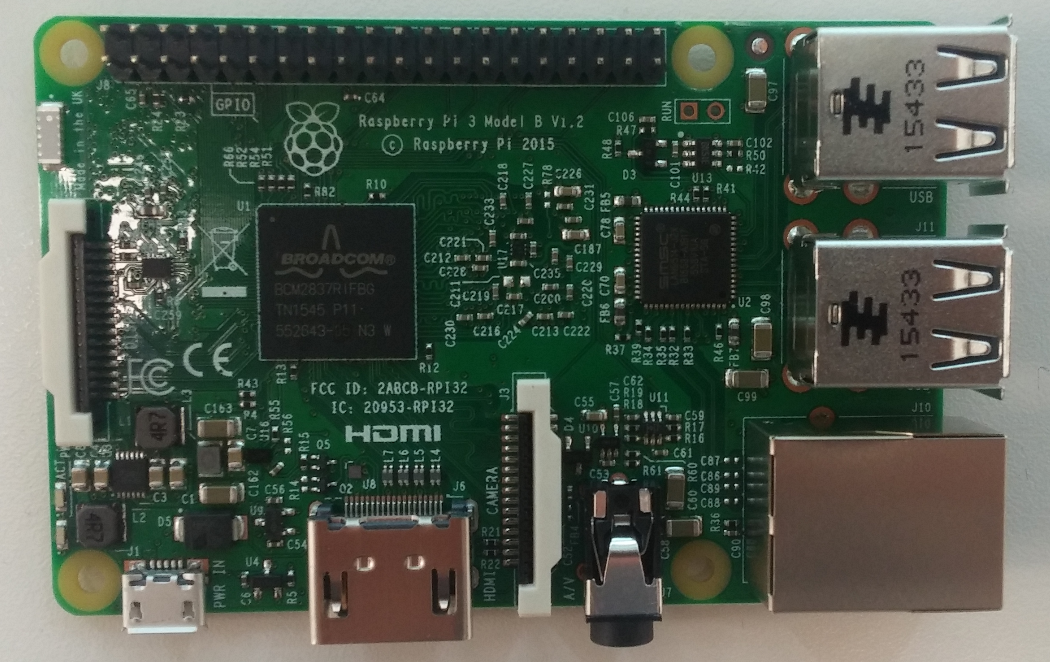
\includegraphics[scale=0.35]{pi3.png}    
    \caption{Raspberry Pi 3}
    \label{fig:piPicture}
\end{figure}

\noindent The Raspberry Pi is the size of a credit card. Model 3 of this was released in February 2016, just in time to become a part of the system set up in this project. This includes a \gls{cpu} speed of 1,2 GHz and 1 GB of \gls{ram}. It is approximately 12 times faster than the first Raspberry Pi. Both Bluetooth and WiFi are included, and it was quite easy to set up, given that the right Linux kernel has been used in the \gls{os} of the Pi. Along with the Raspberry Pi, a good and stable operating system with a kernel that supported the \gls{6lowpan} architecture were needed. For this, Ubuntu Mate version 15.10 with kernel version 4.15 was chosen, and used on the Raspberry Pi. As other versions of Ubuntu, this is Linux based and has a complete \gls{gui} of a full \gls{os}. %The set up of this will be explained in chapter \ref{chp:architecture}.1. 

\subsection{nRF52}

\noindent The most central device of this network is the \gls{microcontroller} used as end-node, the nRF52 developed by Nordic Semiconductor with the \gls{iot} development kit. It is presented as a family of highly flexible, multi-protocol system-on-chip devices\cite{nord}. 


\begin{figure}[ht]
    \centering
    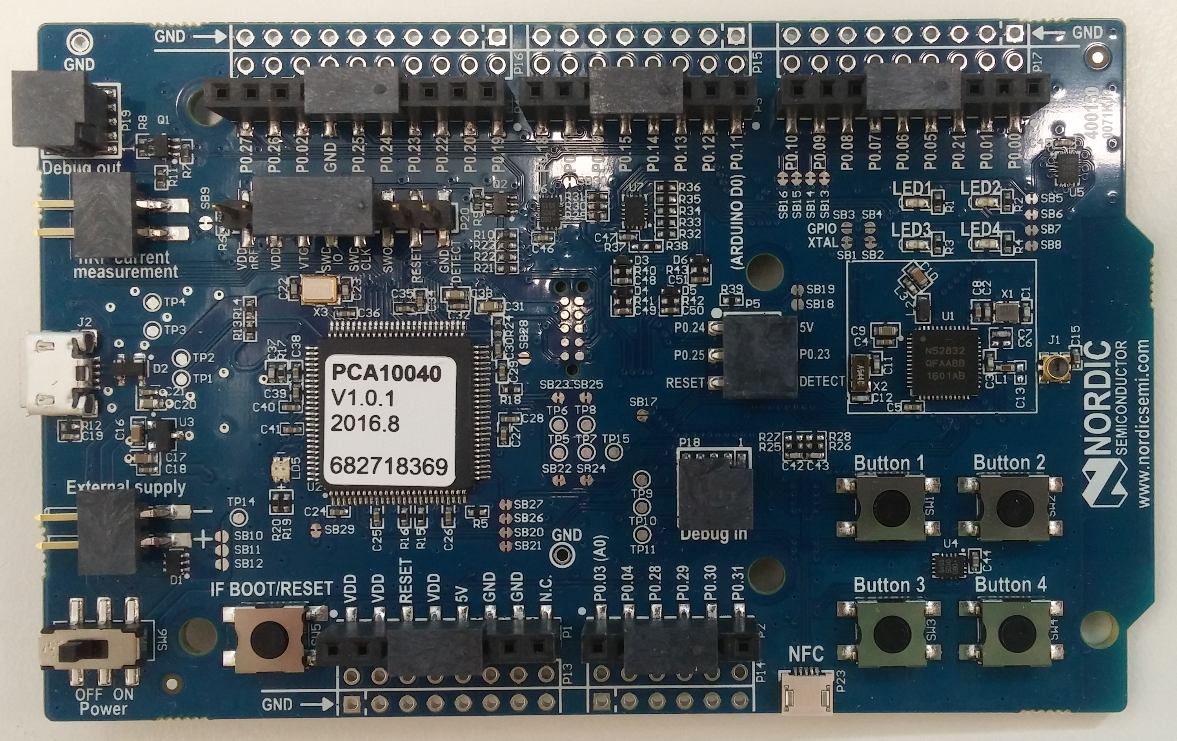
\includegraphics[width=1.0\textwidth]{nRF522.png}    
    \caption{Nordic Semiconductor nRF52 }
    \label{fig:nrf52picture}
\end{figure}


\noindent This device has been advertised as a powerful multiprotocol single chip solution, with both a 32-bit ARM Cortex processor, a 512kB flash, and 64kB of flash memory. The key features mentioned by Nordic Semiconductor \cite{nrf52Nordic} that will be relevant in this network are: 

\begin{itemize}
	\item Multi-protocol 2.4GHz radio
	\item Application development independent from protocol stack
	\item Full set of digital interfaces including \gls{spi} and \gls{i2c}
	\item Low-cost external crystal 32MHz ± 40ppm for Bluetooth, ± 50ppm for ANT
	\item Wide supply voltage range (1.7 V to 3.6 V)
\end{itemize}


\noindent The most interesting points here are the processing power, the flash storage and \gls{ram}, the \gls{i2c} and \gls{spi} buses, and the Bluetooth antenna. In this project, we used three different versions of the \gls{nRF52}, named (from oldest to newest) \textit{PCA10036 V1.0.0, PCA10040 V0.9.0} and \textit{PCA10040 V1.0.1}. All three shows similar results when tested in this system, and Nordic Semiconductor reported that the only significant change is that newer versions should be more stable. Almost all tests in this thesis have been done by using PCA10040 V0.9.0. 

%\cite{nrf52Nordic2}


%\begin{figure}[ht]
%    \centering
%    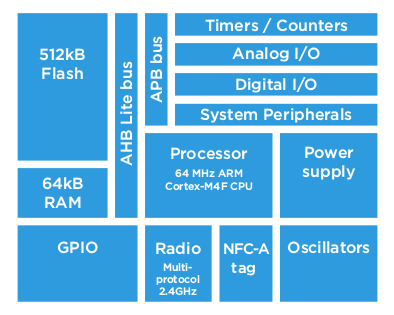
\includegraphics[width=0.5\textwidth]{nrf52Detailed.png}    
%    \caption{Nordic Semiconductor nRF52 chip in detail }
%    \label{fig:nrf52chipDetail}
%\end{figure} 

%\noindent Figure \ref{fig:nrf52chipDetail} shows how the different sections are distributed on the nRF52832 \gls{soc} \ref{fig:nrf52chipDetail}.  

% https://www.nordicsemi.com/Products/nRF52-Series-SoC
\noindent A SoftDevice is a precompiled binary software that implements \gls{ble} on the nRF52. This means that the user can start to work directly in a standard C language interface, which is independent of the Soft Device implementation \cite{softDevice}. This makes it possible for users to write standard programming code instead of requiring a deep knowledge of device-specific configurations. There are several versions of SoftDevices to the nRF52 that can be downloaded from Nordic Semiconductors website\footnote{\url{http://www.nordicsemi.com}}. 


\subsection{Adafruit ADXL345 Accelerometer}

\noindent As seen in the previous section, the nRF52 have several possibilities when it comes to radio communication. In addition to this device, an external sensor was needed to collect data. Supporting both the \gls{i2c} and \gls{spi}, the nRF52 has got most of the standard interfaces needed. Objectives presented in the introduction to this thesis says that it would be preferable both to collect, transport and analyse data in this network. The sensor we chose to do this was the ADXL345 accelerometer from Adafriut \cite{adxlDataSheet}. This was selected for the following main reasons:  

\begin{itemize}
  \item It can measure acceleration in all three axes, X, Y and Z.
  \item It sends digital data immediately, which means no need to use computational power to calculate digital values as needed if the data was captured by an analog accelerometer. 
  \item It supports both \gls{i2c} and \gls{spi}, which makes it possible to connect to the nRF52. 
  \item It supports voltage of 3.3V-5.0V, which fits within the range of output from the nRF52.  
\end{itemize}


%\begin{figure}[ht]
%    \centering
%    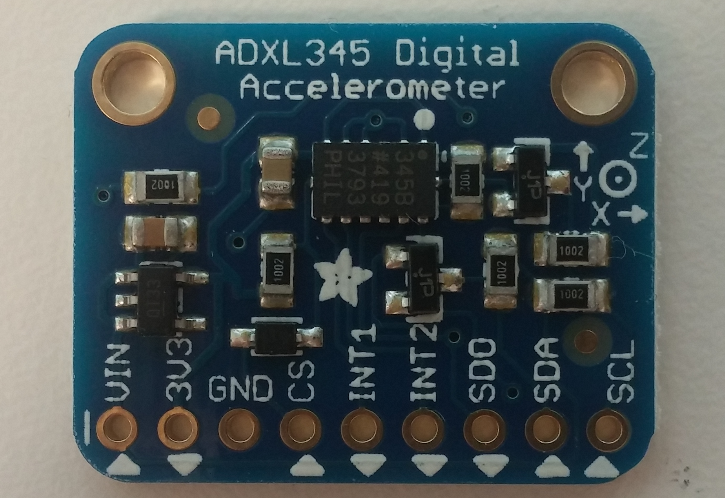
\includegraphics[scale=0.32]{ADXL345.png}    
%    \caption{ADXL345 Accelerometer}
%    \label{fig:adxl345}
%\end{figure}


\begin{figure}[ht]
    \centering
    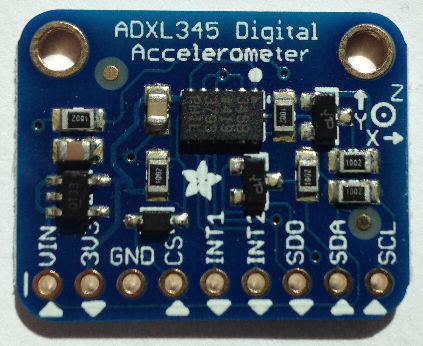
\includegraphics[width=0.5\textwidth]{adxl345imagge}    
    \caption{ADXL345 Accelerometer}
    \label{fig:adxl345}
\end{figure}

\noindent When connecting to the \gls{nRF52}, using the \gls{i2c} interface was chosen because it is simple with few cables, it supports an acceptable bit rate, and several sensors in the same link. 
%Ports VIN, GND, SDA and SCL will be used in this connection, which will be explained in detail in chapter \ref{chp:architecture}. 

\subsection{Additional computational power}

\noindent The devices presented so far are small network devices, reaching from limited computational power to a more powerful central device. These devices can be used as end nodes or more central nodes in an \gls{iot} network. The \gls{Raspberry Pi} has already network connectivity, and can be used as the final node before the results are presented on a screen, a web page, or to be stored on a server. In many cases it will be an advantage to include another node with considerably more computational power before the results are being published. This both limits the computations needed to be done at the \gls{Raspberry Pi} and means that the systems are able to do more deep analyses of the gathered data, without the fear of a system overload. A central stationary computer, a supercomputer or computational power from a web service like \gls{aws} are possible solutions. In this network, a standard stationary computer running a Linux Ubuntu-based system was used as this node. Because of the limited time provided for this thesis, the scope focuses mostly on data analysis and transportation between small nodes in an end-to-end \gls{iot} system. The results were mostly obtained and calculated on the \gls{Raspberry Pi}, meaning this last central node was not extensively used in this solution, but could be a central topic for future projects aiming for a more complex data analysis. 

\subsection{Alternative devices}

An alternative for the Raspberry Pi was never considered since this is a well-known device with a good reputation. This should be easily to use, easy to find advice and help when needed, and easy get hold on devices when needed. There are of course other alternatives available\footnote{For instance the Ardurino Uno, Banana Pi or the BeagleBone Black} that could have been considered if there where any problems with the Raspberry Pi. The main contestant to replace the nRF52 was the Zolertia Z1\footnote{\url{http://zolertia.io/product/hardware/z1-platform}} microcontroller. This was a good alternative to use since it already has got an accelerometer fitted on the board, but does not have the same computational power as the \gls{nRF52}. 

%Should there have been any problems with the nRF52 the Zolertia Z1 would have been a natural contestant as a replacement. ADXL345 is the same accelerometer built in on the Zolertia Z1 microcontroller. This was therefore a natural choise when these two microcontroller where considered the main candidates in the network. If future works will do similar tests later, the results will be comparable between these two. 


\section{Communication technologies}

\noindent After we had chosen the devices to use, the next step was to find relevant communication technologies that could be used to establish a reliable, fast and low power connection between the \gls{nRF52} and the \gls{Raspberry Pi}. 

\subsection{Bluetooth Low Energy}

\noindent \gls{ble}, also known as \textit{Bluetooth Smart}, is a wireless technology for short-range communication developed by the Bluetooth Special Interest Group. The idea was to create a low energy single-hop network solution for \glspl{pan}. A major advantage of this solution is that Bluetooth 4.0 is already a well established technology in cell phones, laptops and several other devices. This means that few changes need to be made to these devices, in order to be able to work with Bluetooth Smart. However, to this date, a device that only implements \gls{ble} is not able to communicate with a device that only implements classic Bluetooth \cite{gomez2012overview}.
The 6LoWPAN Working Group has recognized the importance of \gls{ble} in \gls{iot} \cite{hui2008extending}, as one of the most central technologies in the further development. %\todo{continue from here?} 
%\todo{Denne linken snakker om 6lowpan, flytte til etter jeg har presentert 6LoWPAN?}.

\begin{figure}[ht]
    \centering
    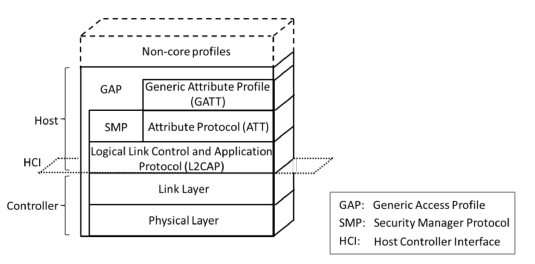
\includegraphics[scale=0.7]{BLEprotocolStack.png}    
    \caption{BLE protocol stack \cite{gomez2012overview}}
    \label{fig:BLEprotocolStack}
\end{figure}

\noindent The protocol stack of \gls{ble} has two main parts, the controller and the host, as shown in \ref{fig:BLEprotocolStack} \cite{gomez2012overview}. In the testbed, the \gls{Raspberry Pi} represents the controller (master), \gls{nRF52} the host (slave). The communication between these components are done through the standard \gls{hci}, a Bluetooth protocol. All slaves are in sleep mode by default and are woken up by the master when these components are needed. Links are being identified by a randomly generated 32-bit code and the \gls{ism} band used is 2,4 GHz \cite{gomez2012overview}. Other protocols include \gls{l2cap} used to multiplex data between higher protocol layers, and the segmentation and reassembly of packets. From here packets are being passed to the \gls{hci}, which is the interface used to communicate between the two \gls{ble} devices. This interface is used in conjunction with \gls{acl}, which is used to create the \gls{tdma} scheme used to transfer packets over the network link, as well as controlling uptime of the end nodes, as this link is set to disconnect automatically after a given time period if there is no activity on the link. Concrete examples of these protocols will be shown later in the thesis.  \textit{BlueZ} Bluetooth protocol stack for Linux \cite{bluez32} was also used on the \gls{Raspberry Pi} in the testbed, to include all the mentioned standard Bluetooth protocols to the Linux kernel. 



\begin{figure}[ht]
    \centering
    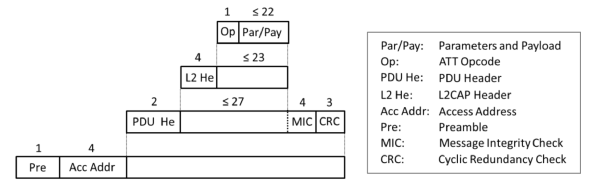
\includegraphics[scale=0.7]{BLEdataUnitStructure.png}    
    \caption{BLE Data Unit Structure \cite{gomez2012overview}}
    \label{fig:BLEdataUnitStructure}
\end{figure}

\newpage
\noindent Figure \ref{fig:BLEdataUnitStructure} shows the data unit structure in \gls{ble}, meaning the different fields that can be used in a packet \cite{gomez2012overview}. The header fields of 4 \glspl{byte} of access addresses and \gls{l2cap} will be central topics of discussion later in this thesis. In the case of the network presented here, when the \gls{ble} slave has been connected to a master, it stops searching for other connectable points. It is not possible for an \gls{nRF52} to connect to several masters, and it will only be possible to create a \textit{star network}, not a \textit{mesh network}. A mesh network would in many cases be preferable since \gls{ble} is considered a \gls{pan} with a very limited range. In a mesh network end-nodes can communicate with each other, meaning they can span a larger area without the need of a central and shared point of connection. Otherwise, \gls{ble} seems like an excellent alternative in this project. 

%Check out: Mikhail Galeev - BLE 

\subsection{6LoWPAN}
%\todo{Write even more in this section?}

\noindent \gls{6lowpan} is a defined protocol for using \gls{ipv6} in low energy networks, to identify sensors and devices over  IEEE 802.15.4, as defined in RFC 4944 \cite{montenegro2007transmission}. To use The Internet Protocol in low energy networks in addition to standard networks was proposed by Geoff Mulligan and the 6LoWPAN Working Group\cite{mulligan20076lowpan}. We chose \gls{6lowpan} because it seemed like a straightforward and smart protocol definition. Since packets in the testbed can end up being forwarded all the way from a \gls{microcontroller} to a central computer through several nodes without being changed, it makes sense to use the same base protocol for all links. In \cite{mulligan20076lowpan}, the advantage of \gls{6lowpan} is explained as not too big to be used in small networks with a small header field, and more flexible to network sized compared to \textit{Zigbee\footnote{\url{http://www.zigbee.org/}}} and \textit{Zensys\footnote{\url{http://www.zensys.com/}}}. As explained in \cite{mulligan20076lowpan}:

\noindent\textit{Utilizing IP  in these networks and pushing it to the very edge of the network devices flattens the naming and addressing hierarchy and  thereby  simplifies  the  connectivity  model. This obviates the need  for  complex  gateways  that,  in  the  past,  were  necessary  to translate   between   proprietary   protocols   and   standard   Internet Protocols and instead can be replaced with much simpler bridges and  routers,  both  of  which  are  well  understood, well  developed and  widely  available  technologies \cite{mulligan20076lowpan}.}


\noindent \gls{6lowpan} was developed to be used in small sensor networks, and implementations can fit into 32Kb flash memory parts. It uses a complex header comparison mechanism that allows the transmission of \gls{ipv6} packets in 4 bytes, much less than the standard \gls{ipv6} 40 bytes. This is achieved by using stacked headers, same as in the \gls{ipv6} model, rather than defining a specific header as for \gls{ipv4}. The device can send only the required part of the stack header, and does not need to include header fields for networking and fragmentation \cite{hui2008extending}. The maximum packet size of the physical layer is set to be 127 bytes \cite{kushalnagar2007transmission}. It is expected from the protocol that other layers will produce packets of the desired size to fit the system. In the example code on the nRF52 in the testbed this is set to 270 bytes for every packet. This will be shown in practical examples and tests later in the thesis. 
%\todo{Double check numbers in this section!}

\subsection{Other alternatives} \label{otherAlternatives}

\noindent \textit{ANT} was the other main alternative to \gls{ble} when network protocols were chosen \cite{ant23}. It also uses the 2,4 GHz ISM band and is made to be used in sensor-based networks. It is supported by the \gls{nRF52}, and could be used with a \gls{Raspberry Pi} if an ANT \gls{usb} dongle is fitted. Using ANT instead would have solved the \gls{ble} problem not being able to connect several devices together in a mesh network, since ANT supports this. Other than this the difference is small. \gls{ble} is, on the other hand, backed up by other mobile devices, meaning it is possible to use a mobile application developed by Nordic Semiconductor to test the connection. One of the main intentions from \gls{item}, when the problem description was written was to test \gls{ble} in such a setting. Because of this argument, we chose \gls{ble}. 



\noindent Two other contestants other than \gls{6lowpan}, were \textit{Zigbee} and \textit{Zensys}. These are compared directly in \cite{mulligan20076lowpan}. The major factors here are that \gls{6lowpan} has a network size bigger than the others. It supports Internet connectivity using routers, the use of \gls{udp} and \gls{tcp}, low amounts of \gls{ram} and small headers \cite{mulligan20076lowpan}. 

%\todo{add numbers, 2in64th compared to the others}


\section{Transport protocols}

\noindent To transfer data from the end nodes to the central points of the network, either for analysing or already analysed data, a fast, efficient and stable transport protocol has to be used. This is a central aspect of the testbed because the limitations of the sending rate are assumed to be one of the main constraints for network throughput, either in the form of limits of data at once or number of transmissions per second. The protocol needs to be stable and energy efficient and work with both \gls{ble} and \gls{6lowpan}. Nordic Semiconductor provides example code and examples on how to get started with this, having been used as the basis for this work.

\subsection{CoAP}

%The \\ protocol is described in the documentation as follows: 
 
\noindent \gls{coap} is a transport protocol designed to be used in constrained networks for \gls{m2m} communication. It is \gls{udp} based and works well in low-power and lossy networks. It can be used with \glspl{microcontroller}, and with \gls{ipv6} and \gls{6lowpan}. Both GET and PUSH functionalities are available, as well as \textit{observable} GET. Other commands used in \gls{coap} are GET, PUT, POST and DELETE, to get or change data. This means that a server can "subscribe" to end nodes in the network, and get updates either after a given time span or when there have been changes made to a followed field. Therefore, this seemed like a promising protocol and was chosen as the main transport protocol in the network test\cite{shelby2014constrained}. The main technical features described in \gls{coap} include fulfilling \gls{m2m} requirements, support of asynchronous messages, \gls{udp} based communication and stateless mapping to \gls{http}. 

\noindent CoAP has several similarities with \gls{http}, using the same client and server roles. A client sends a request, and the server sends a response back. Many of the response-codes are also very similar, with \textit{404: Not found} as the best known. In \gls{m2m} communication, both participants sometimes need to be both client and server, and the \gls {coap} protocol handles this with a two-layer approach. There are four different main \glspl{messageType} defined in \gls{coap} \cite{shelby2014constrained}. 

%\todo{make figure of CoAP Layering}.

\begin{itemize}
	\item A Confirmable message, \gls{con}, requires one \gls{ack} for every message received. If a message is not received correctly, the receiver will ask for exactly one return message of the type Acknowledgement. 
	\item A Non-confirmable message, \gls{non}, does not require an \gls{ack}. This may result in a higher possibility of a packet getting lost, especially in lossy networks, but it requires less capacity from the network and should, in general, be faster. 
	\item An Acknowledgement confirms that a specific \gls{con} packet has reached its destination. 
	\item A Reset message tells the sender that a specific message was received, but some content is missing to be able to understand it fully. For instance, if the receiver has had a reboot during the transmission. 
	\item An empty Reset message represents a ping test of \gls{rtt}, which we will use when testing a connection. 
\end{itemize}
       


\begin{figure}[ht]
    \centering
    \includegraphics[scale=0.6]{CONclientserver.png}    
    \caption{CON CoAP set up sequence diagram \cite{shelby2014constrained}}
    \label{fig:CONOackSeqDiagram}
\end{figure}

 

\begin{figure}[ht]
    \centering
    \includegraphics[scale=0.6]{NONOackSeqDiagram2.png}    
    \caption{NON CoAP set up sequence diagram \cite{shelby2014constrained}}
    \label{fig:NONOackSeqDiagram}
\end{figure}

\noindent Figure \ref{fig:CONOackSeqDiagram} shows the basic message sequence between the client and the server in a \gls{coap} \gls{con} network. Every \gls{con} request message needs to get an \gls{ack} back.

\noindent Figure \ref{fig:NONOackSeqDiagram} shows the same for \gls{non}, where no \glspl{ack} are required. The same initial set up with \gls{con} and \gls{ack} messages are still needed, to establish a connection between the client and server before a stream of \gls{non}-messages can be sent. We here get a less reliable connection than using \gls{con}, since messages can be dropped without either the client or the server gets notified. Systems where a few packets can be lost without difficulties, for instance in a sensor based network like the network presented in this thesis, can use this as an advantage. A message ID is still provided to every message to remove duplicated messages, but dropped messages are lost data.  This is not a good solution if the sent packages contained data that could not be dropped. For instance, containing crucial patient information from sensors on a patient's body. The more reliable solution \gls{con} is a better alternative in this case. These differences are the same as being experienced in the \gls{iot} system described in this thesis, which can be seen in figure \ref{fig:CoAPNONwiresharkSetUp}. A \gls{con} message is sent several times, to set up the initial connection. When an \gls{ack} is received as a response, the continuous transportation of \gls{non}-packets without \glspl{ack} can begin. %\todo{Comment: Okey, but not clear why for the last part. Change?} 

\begin{figure}[ht]
    \centering
    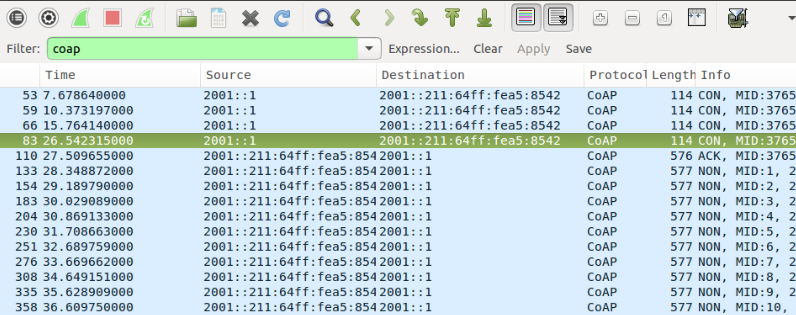
\includegraphics[width=1.0\textwidth]{coapCONwiresharksetUpSequence.png}    
    \caption{CoAP NON, set up sequence, Wireshark capture}
    \label{fig:CoAPNONwiresharkSetUp}
\end{figure}

%\todo{Show examples of setting up coap NON needs acks first? Wireshark without bluetooth-sniffing?}

\noindent The message format used in \gls{coap} is very simple, as seen in figure \ref{fig:CoAPMessageFormat}. The four first byte are header files, followed by optional tokens and options. When these are not being used, like in the testbed, the minimal header size will be 4 bytes\cite{shelby2014constrained}. The rest can be used for a variable sized \gls{payload}. A small header size is a huge advantage in \gls{iot} networks.

%\todo{Change figure to include bytes}
\newpage
\begin{figure}[h!]
    \centering
    \includegraphics[width=1.0\textwidth]{CoAPMessageFormat3.png}    
    \caption{CoAP message format \cite{shelby2014constrained}}
    \label{fig:CoAPMessageFormat}
\end{figure}



%\begin{figure}[ht]
%    \centering
%    \includegraphics[scale=0.6]{CoAPUsageOfMessageTypes.png}    
%    \caption{CoAP usage of message types}
%    \label{fig:CoAPUsageOfMessageTypes}
%\end{figure}



\subsection{MQTT}

\noindent An alternative transport protocol in a system such as this is \gls{mqtt}. This is  known as a publish-subscribe messaging system based on \gls{tcp} for \gls{m2m} communication. A client will in this case \textit{subscribe} to a \textit{publisher} in the network \cite{hunkeler2008mqtt}. When a publisher updates a field of interest for the subscriber, the subscriber will get notified. Subscriptions are being coordinated by a \textit{broker}, as seen in figure \ref{fig:mqttSeqDiagram}. Messages sent in such a network are either \textit{sub(topic)} to subscribe to a topic, or \textit{pub(topic, data)} to publish data \cite{mqttWebsite}. 


\begin{figure}[ht]
    \centering
    \includegraphics[width=0.8\textwidth]{mqttSeqDiagram.png}    
    \caption{MQTT subscription sequence diagram \cite{hunkeler2008mqtt}}
    \label{fig:mqttSeqDiagram}
\end{figure}

\noindent \gls{mqtt} supports end-to-end \gls{qos} and has a simple and effective message architecture. This protocol would also be possible to use in the testbed. Because of the limited time frame of this thesis, it was decided to study \gls{coap} in depth first, and leave the testing of \gls{mqtt} to future work. 


%\newpage
\section{Software tools}

\noindent As an \gls{ide}, we used \textit{KEIL Vision}, as recommended by Nordic Semiconductor in \cite{nord}, for writing C programming code. For other programming languages, (for instance Python 3.4), we used Sublime Text 2 for Windows and Linux, as well as \textit{Pluma} for Ubuntu Mate on the Raspberry Pi. 

\noindent Wireshark is a software tool used to analyse networks and capture packets sent with different technologies \cite{lamping2004wireshark}. Later, the data can be filtered and analysed, for instance by filtering out all packets except \gls{coap} and \gls{ble}, which we used in this case. Wireshark has been one of the most valuable tools to be able to analyse data to such an extent as done in this thesis. An example of use is shown in figure \ref{fig:CoAPNONwiresharkSetUp}. 

\noindent \textit{Copper}\cite{copper3} is a generic browser which can be extended to a standard \textit{Firefox} browser. It is made to be used in \gls{iot} networks based on \gls{coap}, just like this network. Using Copper, it was easy to use GET and PUT messages, as well as observing a server by using a simple \gls{gui}. By removing the need of using terminal commands and programming scripts, this makes the system easier to use with less development effort outside the scope of this thesis. An example of the \gls{gui} can be seen in figure \ref{fig:copperExample} 
\cite{kovatsch2011demo}.

\begin{figure}[ht]
    \centering
    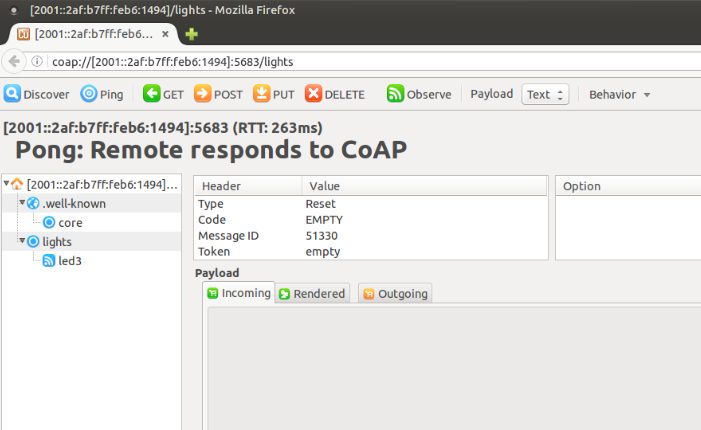
\includegraphics[width=1.0\textwidth]{CopperExample.png}    
    \caption{Copper example}
    \label{fig:copperExample}
\end{figure}

\newpage

\noindent \gls{radvd} is a software tool that can be used to advertise \gls{ipv6} addresses in a local network, using \gls{ndp} \cite{chown2011rogue}. It is being used to multicast and forward packets in this network. When a packet is sent from an end node to another, the communication needs to go through the central point in the star network, the Raspberry Pi in this case. Here, \gls{radvd} ensures that the packages are being routed to the right end-point, meaning the right nRF52 in the testbed. To make the most basic figures in this thesis the web-based tool \textit{\url{http://draw.io}} was used. \textit{\url{http://polt.ly}} was used to draw the graphs used.  


